%%%%%%%%%%%%%%%%%%%%%%%%%%%%%%%%%%%%%%%%%%%%%%%%%%%%%%
% A Beamer template for University of Wollongong     %
% Based on THU beamer theme                          %
% Author: Qiuyu Lu                                   %
% Date: July 2024                                    %
% LPPL Licensed.                                     %
%%%%%%%%%%%%%%%%%%%%%%%%%%%%%%%%%%%%%%%%%%%%%%%%%%%%%%
% Customized for Sharif University of Technology     %
%%%%%%%%%%%%%%%%%%%%%%%%%%%%%%%%%%%%%%%%%%%%%%%%%%%%%%


\documentclass[serif, aspectratio=169]{beamer}
%\documentclass[serif]{beamer}  % for 4:3 ratio
\usepackage[T1]{fontenc} 
\usepackage{fourier} % see "http://faq.ktug.org/wiki/uploads/MathFonts.pdf" for other options
\usepackage{hyperref}
\usepackage{latexsym,amsmath,xcolor,multicol,booktabs,calligra}
\usepackage{graphicx,pstricks,listings,stackengine}
\usepackage{lipsum}
\usepackage{booktabs}
%\usepackage{geometry}
\usepackage{tabularx}
\author{Ali Sharifi-Zarchi}
\title{Machine Learning (CE 40717)}
\subtitle{Fall 2024}
\institute{
    CE Department \\
    Sharif University of Technology
}
%\date{\small \today}
% \usepackage{UoWstyle}
\usepackage{SUTstyle}

% defs
\def\cmd#1{\texttt{\color{red}\footnotesize $\backslash$#1}}
\def\env#1{\texttt{\color{blue}\footnotesize #1}}
\definecolor{deepblue}{rgb}{0,0,0.5}
\definecolor{deepred}{RGB}{153,0,0}
\definecolor{deepgreen}{rgb}{0,0.5,0}
\definecolor{halfgray}{gray}{0.55}

\lstset{
    basicstyle=\ttfamily\small,
    keywordstyle=\bfseries\color{deepblue},
    emphstyle=\ttfamily\color{deepred},    % Custom highlighting style
    stringstyle=\color{deepgreen},
    numbers=left,
    numberstyle=\small\color{halfgray},
    rulesepcolor=\color{red!20!green!20!blue!20},
    frame=shadowbox,
}

\begin{document}

\begin{frame}
    \titlepage
    \vspace*{-0.6cm}
    \begin{figure}[htpb]
        \begin{center}
            
\includegraphics[keepaspectratio, scale=0.25]{pic/sharif-main-logo.png}
        \end{center}
    \end{figure}
\end{frame}

\begin{frame}    
\tableofcontents[sectionstyle=show,
subsectionstyle=show/shaded/hide,
subsubsectionstyle=show/shaded/hide]
\end{frame}

\section{Optimization}
\subsection{Problem Definition}

\begin{frame}{Problem Definition}
    \begin{itemize}%[<+-| alert@+>] % stepwise alerts
        \item \textbf{Goal}: Given a function $f(x)$ of some variable $x$, find the value of $x$ where $f(x)$ is minimum or maximum
        \item In neural networks, the goal is to make the prediction error as small as possible
        \item We want to find the network weights $W^*$ that result in the lowest loss
    \end{itemize}
    
    \[
    \mathcal{L} = \frac{1}{N} \sum_{i=1}^{N} \ell(y_i, \hat{y}_i)
    \]
    \[
    \mathbf{W}^* = \arg\min_{\mathbf{W}} \frac{1}{N} \sum_{i=1}^{n} \ell(y_i, \hat{y}_i)
    \]
\end{frame}
\begin{frame}{Problem Definition}
    \begin{itemize}
        \item Simply put, we want to find the direction to step in that will \textbf{reduce our loss} as quickly as possible
        \item In other words, \textbf{which way is downhill?}
    \end{itemize}
\end{frame}

\subsection{Convexity and Optimization}
\begin{frame}{Convexity and Optimization}
    \begin{minipage}{0.6\linewidth}
        \begin{itemize}
            \item \textbf{Definition}: A function is \textbf{convex} if, for any two points on the curve, the line segment connecting them lies above or on the curve
            \begin{itemize}
                \item \textbf{Example}: Bowl-shaped curves
            \end{itemize}
            \item \textbf{Convex functions} are easier to optimize because they have only \textbf{one global minimum} (the lowest point)
            \begin{itemize}
                \item Analytical solutions $(\nabla f(x) = 0)$ and second-order methods $(\nabla^2 f(x) > 0)$ can be used for faster and more accurate convergence
                \item \textbf{Gradient descent} is guaranteed to converge to the global minimum in convex functions
            \end{itemize}
        \end{itemize}
    \end{minipage}%
    \hfill
    \begin{minipage}{0.4\linewidth}
        \centering
        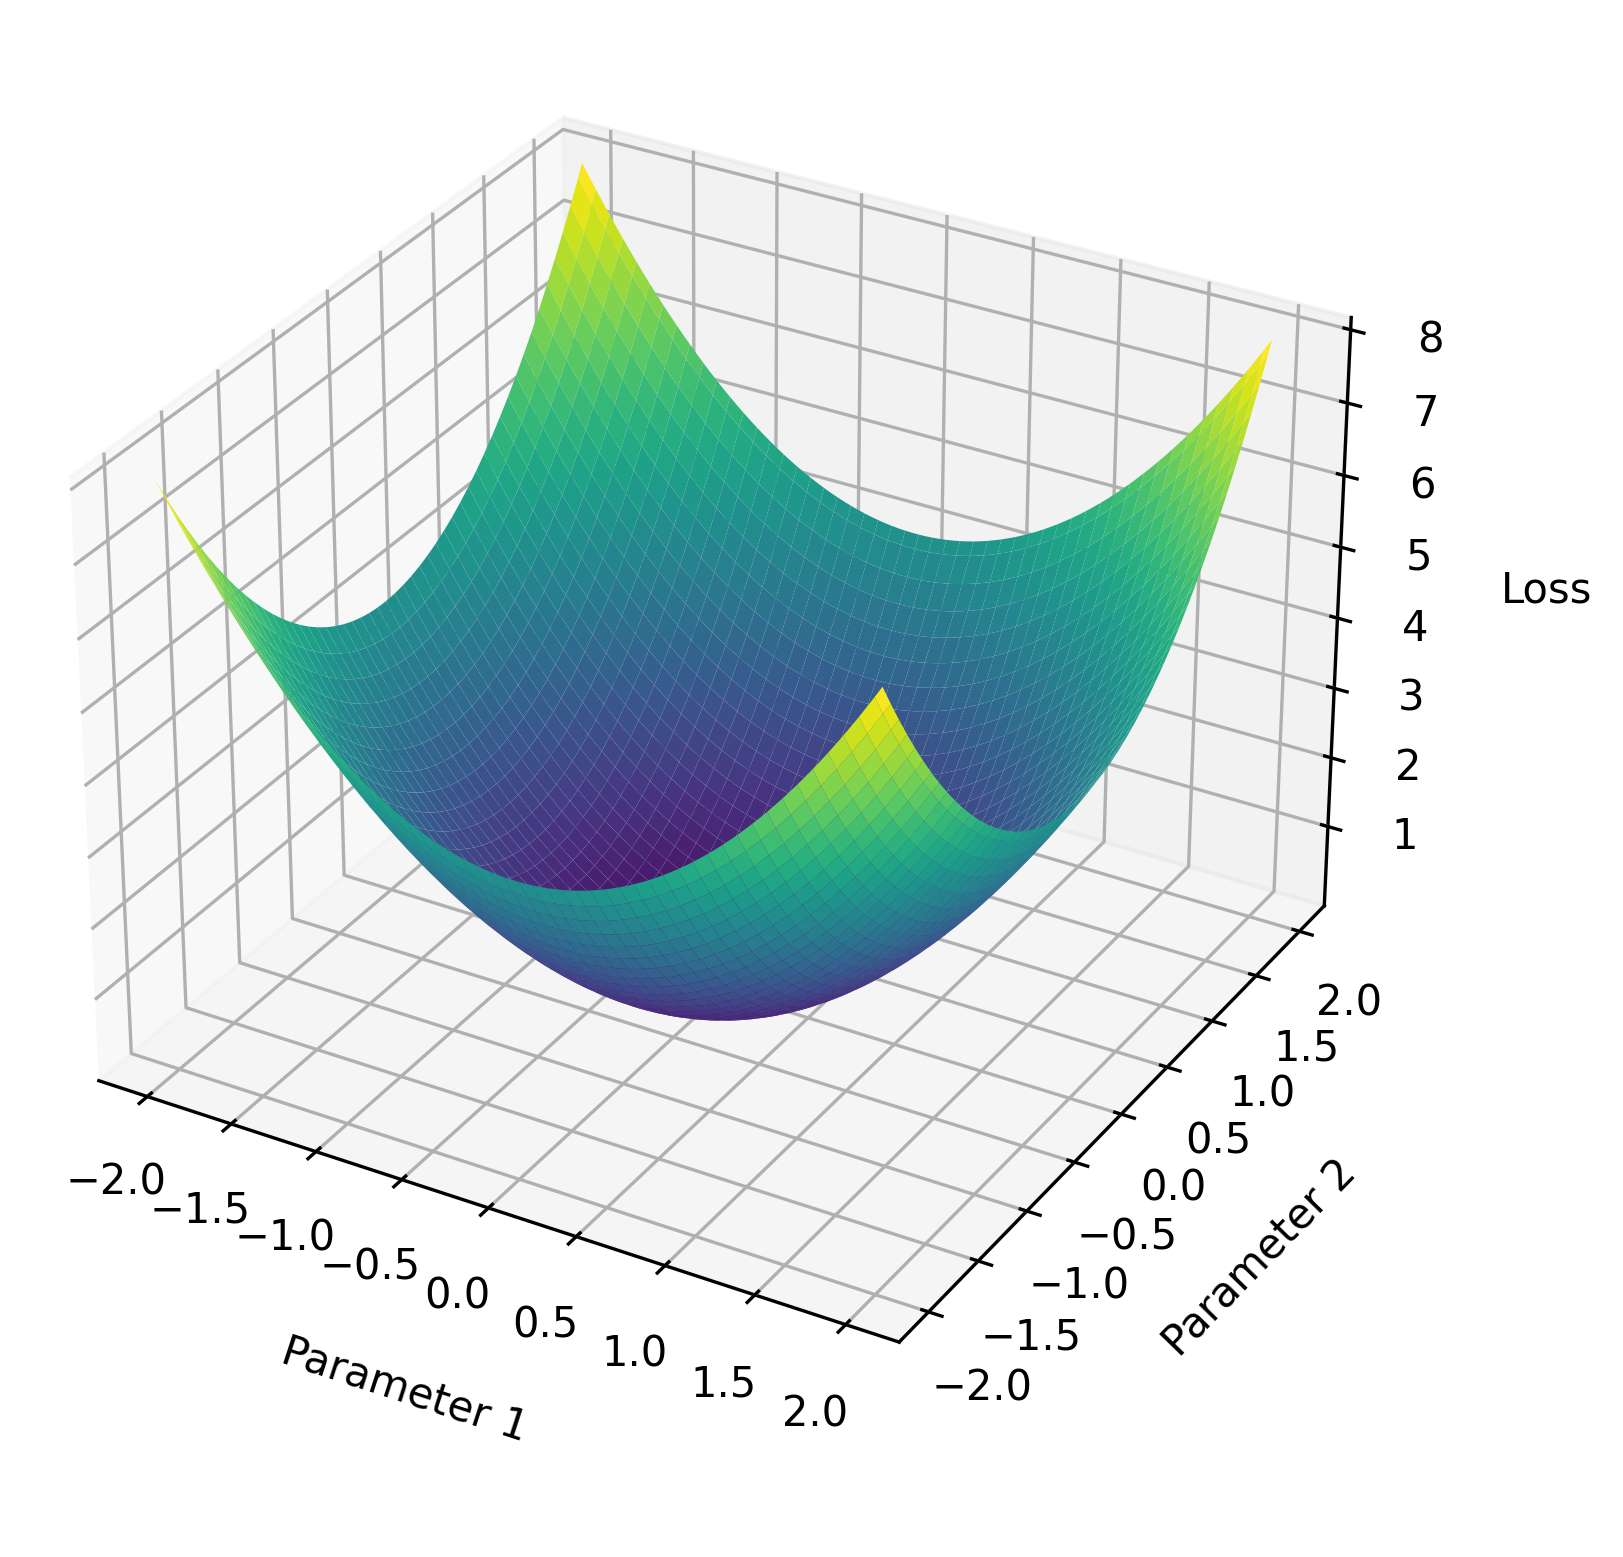
\includegraphics[height=.6\textheight]{pic/loss_convex.jpg}
    \end{minipage}
\end{frame}

\begin{frame}{Convexity and Optimization}
    \begin{itemize}
        \item \textbf{Definition}: a function is \textbf{non-convex} if it has multiple local minima and maxima
        \begin{itemize}
            \item \textbf{Global Minimum}: The very lowest point across the whole curve
            \item \textbf{Local Minimum}:  A point that's lower than nearby points, but not the lowest overall
            \item \textbf{Saddle Points}: A flat region where the slope is almost zero. It can go up in some directions and down in others
        \end{itemize}
        \item Non-convex functions make finding the \textbf{global minimum} complicated
    \end{itemize}
    \begin{center}
        \begin{minipage}{0.5\linewidth}
            \centering
            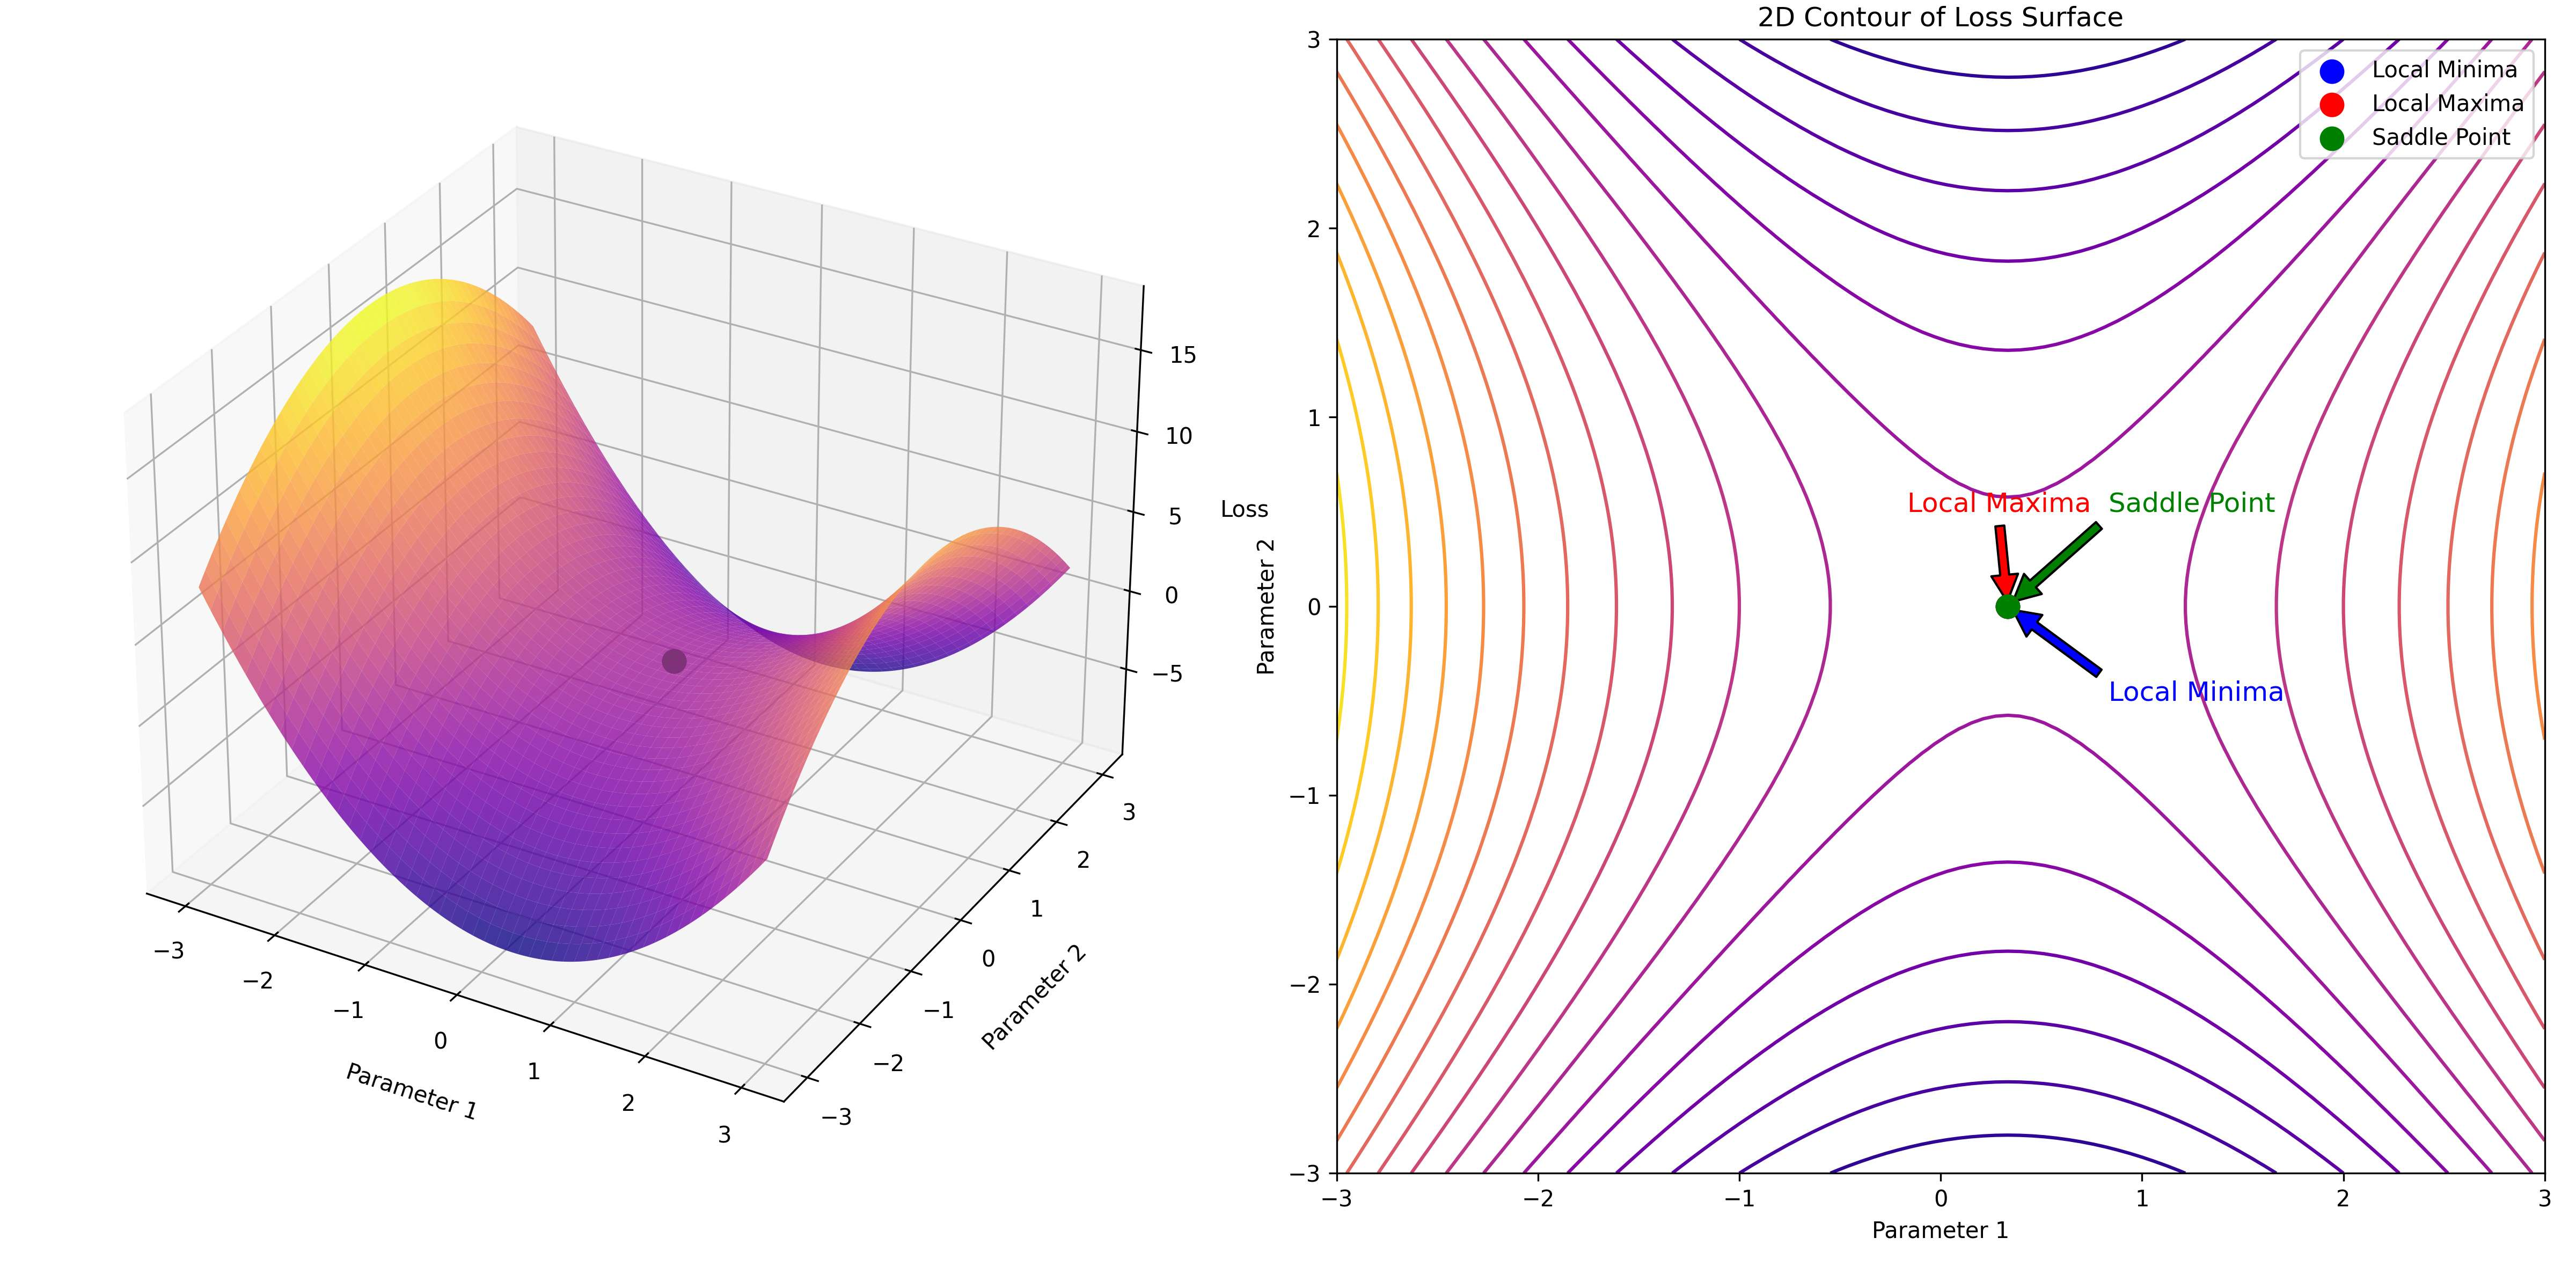
\includegraphics[height=.5\textheight]{pic/Saddle_point.jpg}
        \end{minipage}
    \end{center}
\end{frame}

\section{The Loss Surface}
\begin{frame}{Definition}
\begin{minipage}{0.5\linewidth}
    \begin{itemize}
        \item The loss surface represents how the error changes based on the network's weights
        \item The loss surface of a neural network is typically \textbf{non-convex} due to multiple layers, nonlinear activation functions, and complex interactions between parameters, resulting in multiple local minima and saddle points
        \item In large networks, most local minima give similar error values and are close to the \textbf{global minimum}. This isn't true for smaller networks
    \end{itemize}
\end{minipage}%
%\begin{center}
\begin{minipage}{0.5\linewidth}
    \begin{figure}[h]
        \centering
        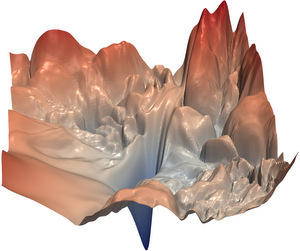
\includegraphics[height=.5\textheight]{pic/resnet56_noshort_small.jpg}
        \caption{\footnotesize ResNet56 from \url{https://github.com/tomgoldstein/loss-landscape}}
    \end{figure}
\end{minipage}
%\end{center}
\end{frame}

\begin{frame}{Loss Optimization}
    \begin{minipage}{0.5\linewidth}
    \begin{itemize}
        \item How can we optimize a non-convex loss function?
        \item \textbf{Strategy}: Instead of randomly searching for a good direction, we calculate the \textbf{best direction} to reduce the loss
        \begin{itemize}
            \item  This is mathematically guaranteed to be the direction of the steepest descent
        \end{itemize}
    \end{itemize}
    \end{minipage}%
    \begin{minipage}{0.5\linewidth}
        \begin{figure}[h]
            \centering
            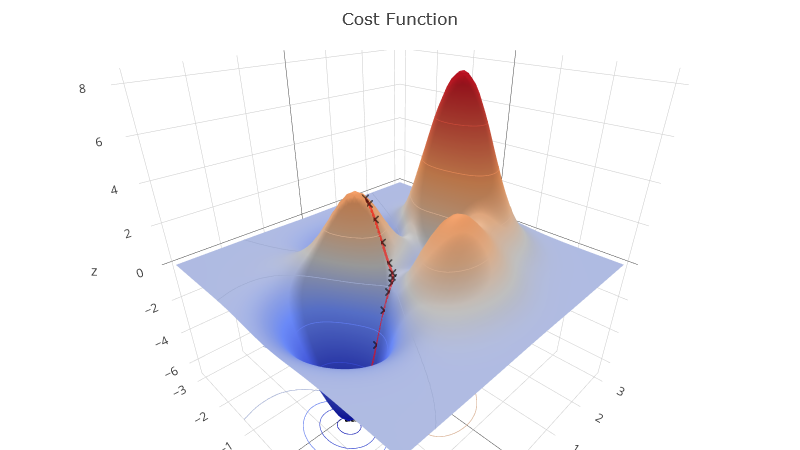
\includegraphics[height=.6\textheight]{pic/gradient_descent_blog.skz.dev.png}
            \caption{\footnotesize Gradient Descent visualization from \url{https://blog.skz.dev/gradient-descent}}
        \end{figure}
    \end{minipage}
\end{frame}


\section{Gradient Descent}
\subsection{Recap of Gradient Descent}
\begin{frame}{Gradient Descent}
    \begin{itemize}
        \item As introduced earlier, Gradient Descent is an iterative method for minimizing the error by updating network weights in the direction of the steepest descent (negative gradient)
        \[\theta_{t} = \theta_{t-1} - \eta \nabla_{\theta} J(\theta)\]\\
        where:
        \begin{itemize}
            \item $\eta$ is called the 'learning rate' or 'step size'
        \end{itemize}
        \item The goal is to keep adjusting the weights until we reach a point where the error is as low as possible (a local or global minimum)
    \end{itemize}
\end{frame}

\begin{frame}{Types of Gradient Descent}
    \begin{itemize}
        \item \textbf{Batch Gradient Descent}: Uses the entire dataset to calculate the gradient. This gives smooth updates but can be slow
        \item \textbf{Stochastic Gradient Descent (SGD)}: Uses one data point at a time, leading to faster but noisier updates
        \item \textbf{Mini-batch Gradient Descent}: Uses small groups (batches) of data points. This is a balance between batch and stochastic, combining speed with more stable updates
    \end{itemize}
\end{frame}

\begin{frame}{Types of Gradient Descent}
\begin{table}[h!]
\centering
\begin{tabularx}{\textwidth}{@{} lX X @{}}
\toprule
\textbf{Type} & \textbf{Advantages} & \textbf{Disadvantages} \\ 
\midrule
\textbf{Batch}   & 
Stable convergence \newline 
Accurate gradient estimate  & 
Computationally expensive \newline 
Slow for large datasets \\ 
\midrule
\textbf{Stochastic (SGD)}   & 
Fast updates \newline 
Can escape local minima & 
Noisy updates \newline 
May not converge smoothly \\ 
\midrule
\textbf{Mini-Batch}   & 
Faster than batch, more stable than SGD \newline 
Efficient for larger datasets & 
Requires tuning batch size \newline 
Some noise remains \\ 
\bottomrule
\end{tabularx}
\caption{\footnotesize Comparison of Gradient Descent Types}
\end{table}
\end{frame}

\subsection{Problems with SGD}
\begin{frame}{Problem 1 with SGD}
    \begin{itemize}
        \item \textbf{SGD} is fast and can escape local minima, but it faces some issues
        \item What if the loss changes quickly in one direction but slowly in another?
        \begin{itemize}
            \item \textbf{Slow} progress along the shallow dimension, \textbf{jitter} along the steep direction
        \end{itemize}
    \end{itemize}
    \hfill
    \hfill
 %   \begin{minipage}{0.5\textwidth}
    \begin{center}
        \begin{figure}
            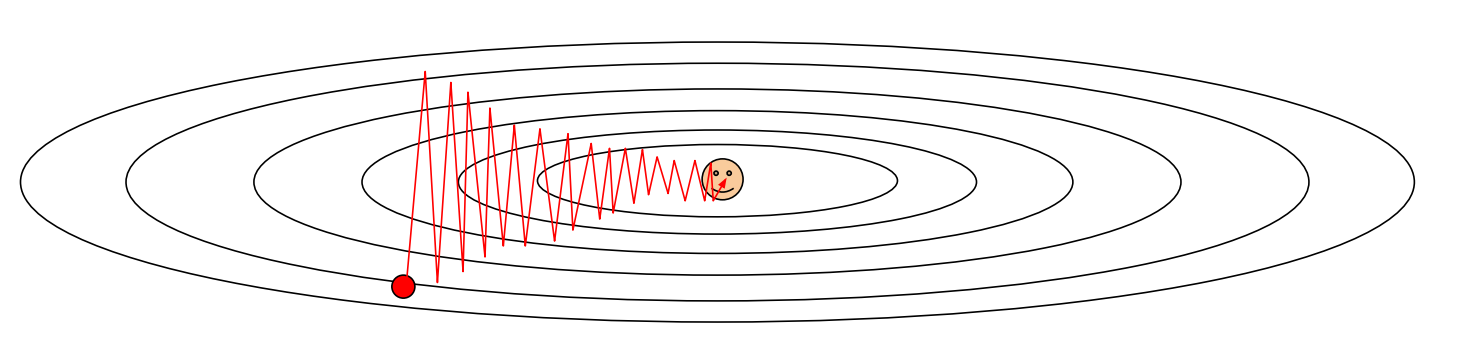
\includegraphics[width=1\linewidth]{pic/sgd_stanford.png}
            \caption{\footnotesize SGD visualization from CS231n: Convolutional Neural Networks for Visual Recognition}
        \end{figure}
    \end{center}
 %   \end{minipage}
\end{frame}

\begin{frame}{Problem 2 with SGD}
    \begin{minipage}{0.4\textwidth}
        \begin{itemize}
        \item What if the loss function has a local minima or saddle point?
        \begin{itemize}
            \item The algorithm may settle for \textbf{sub-optimal solutions} or take a \textbf{long time} to make significant progress
        \end{itemize}
        \end{itemize}
    \end{minipage}%
    \begin{minipage}{0.6\textwidth}
        \centering
        \begin{center}
        \begin{figure}
        \centering
            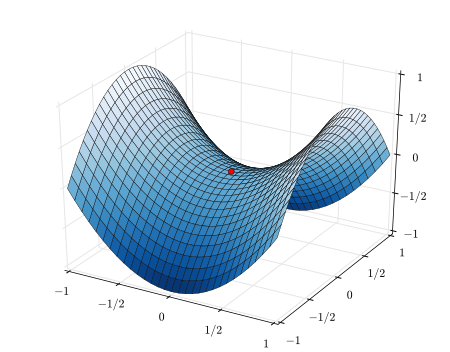
\includegraphics[width=0.75\linewidth]{pic/saddle_wiki.png}
            \caption{\footnotesize Saddle point from \url{https://en.wikipedia.org/wiki/Saddle_point}}
        \end{figure}
        \end{center}
    \end{minipage}
\end{frame}

\begin{frame}{Problem 3 with SGD}
    \begin{minipage}{0.4\textwidth}
        \begin{itemize}
        \item Gradients that come from single data points or mini-batches can be \textbf{noisy}
        \end{itemize}
    \end{minipage}%
    \begin{minipage}{0.6\textwidth}
        \centering
        \begin{figure}
            \centering
            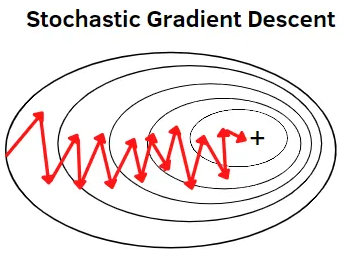
\includegraphics[width=0.6\linewidth]{pic/sgd_mlexplained.png}
            \caption{\footnotesize SGD visualization from \url{https://laptrinhx.com/understanding-optimization-algorithms-3818430905/}}
        \end{figure}
    \end{minipage}
\end{frame}

\begin{frame}{Problem 4 with SGD}
    \begin{itemize}
        \item Using the same learning rate for all dimensions can lead to:
        \begin{itemize}
            \item Smooth convergence in some directions
            \item Oscillations or divergence in other directions
        \end{itemize}
        \item \textbf{Proposal}:
        \begin{itemize}
            \item Track oscillations in each direction
            \item Increase steps in stable directions
            \item Decrease steps in oscillating directions
        \end{itemize}
    \end{itemize}
\end{frame}


\begin{frame}{Problem Definition}
    \begin{itemize}
        \item \textbf{Goal}: Choose an appropriate learning rate to avoid slow convergence and getting stuck in local minima while not overshooting or becoming unstable
        \item \textbf{Naive Approach}: Try lots of different learning rates and see what works "just right"
        \begin{itemize}
            \item This can be inefficient and time-consuming
        \end{itemize}
        \item \textbf{Smarter Approach}: Design an adaptive learning rate that adapts to the loss surface
        \begin{itemize}
            \item We can achieve this by incorporating \textbf{Momentum}
        \end{itemize}
    \end{itemize}
    \vfill
    \begin{center}
        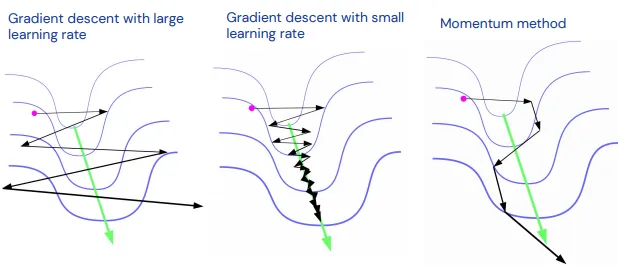
\includegraphics[width=0.6\linewidth]{pic/compare_momentum.png}
    \end{center}
\end{frame}

\section{Momentum}
\begin{frame}{Momentum}
    \begin{minipage}{0.5\textwidth}
        \begin{itemize}
            \item \textbf{Goal}: Speed up convergence by using past gradients to smooth out oscillations and avoid getting stuck
            \begin{itemize}
                \item Keep moving in the same general direction as previous steps
            \end{itemize}
            \item \textbf{Benefit}: Accelerates learning in important directions while reducing oscillations in irrelevant ones
        \end{itemize}
    \end{minipage}%
    \begin{minipage}{0.5\linewidth}
    \begin{figure}[h]
        \centering
        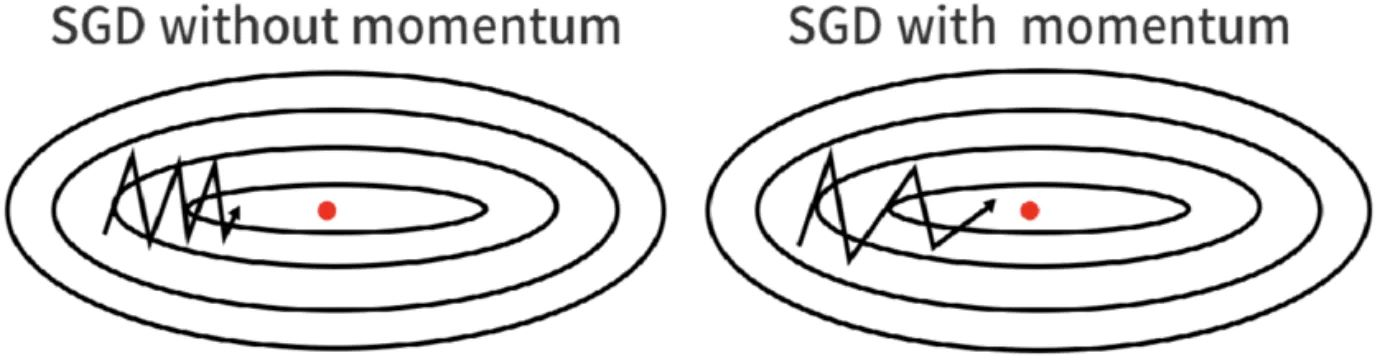
\includegraphics[height=.25\textheight]{pic/momentum_paperswithcode.jpg}
        \caption{\footnotesize SGD comparison from \url{https://paperswithcode.com/method/sgd-with-momentum}}
    \end{figure}
    \end{minipage}
\end{frame}


\begin{frame}{First Momentum}
    \begin{itemize}
        \item The first momentum, denoted as $m_t$, is essentially \textbf{the moving average of the gradients}
         \item It’s inspired by physics: like a ball rolling in a frictionless bowl, it keeps moving due to accumulated momentum
        \item In gradient descent with momentum, the update rule is:
        \[m_t = \beta_1 m_{t-1} + (1 - \beta_1) \nabla_{\theta}J(\theta_{t-1})\]
        \[\theta_t = \theta_{t-1} - \eta m_t\]\\
        where:
        \begin{itemize}
            \item $m_t$ is the first moment
            \item $\beta_1$ (momentum term) controls how much of the past gradients to include (typically 0.9 or 0.99)\\
            \item $\eta$ is the learning rate\\ 
            \item $\nabla_{\theta}J(\theta_t)$ is the gradient of the cost function
        \end{itemize}
    \end{itemize}
\end{frame}

\begin{frame}{Second Momentum}
    \begin{itemize}
        \item The second momentum, denoted as $v_t$, is \textbf{the moving average of the squared gradients} It tracks the magnitude of the gradients over time
        \item This is updated similarly to the first momentum:
        \[v_t = \beta_2 v_{t-1} + (1 - \beta_2) (\nabla_{\theta} J(\theta_t) \odot \nabla J(\theta_t)\]
        \[\theta_t = \theta_{t-1} - \eta v_t\]
        where:
        \begin{itemize}
        \item $v_t$ is the second moment% (uncentered variance, squared gradients)
        \item$\beta_2$ is the decay rate
        \item$\eta$ is the learning rate
        \item$\nabla_{\theta}J(\theta_t)$ is the gradient of the cost function
        \item $\odot$ denotes the element-wise (Hadamard) product
        \end{itemize}
    \end{itemize}
\end{frame}

\begin{frame}{Moment Bias Correction}
    \begin{itemize}
        \item \textbf{Problem}: When we start training, both $m_t$ and $v_t$ are initialized to zero. This means that the estimates for the first and second moments will be biased toward zero, especially during the initial steps when the gradients are still small
        \item \textbf{Solution}: To counteract this initial bias, we use the bias-corrected versions of $m_t$ and $v_t$:
        \[\hat{m}_t = \frac{m_t}{1 - \beta_1^t}, \quad 
        \hat{v}_t = \frac{v_t}{1 -\beta_2^t}\]
    \end{itemize}
\end{frame}

\begin{frame}{Momentum update}
    \begin{minipage}{0.5\textwidth}
    \begin{itemize}
    \item Momentum update steps involve two stages:
    \begin{enumerate}
        \item Take a step in the opposite direction of the gradient at the current position
        \item Add a scaled version of the previous step to this move
    \end{enumerate}
    \item Reversing these steps leads to a more optimal approach, known as \textit{Nesterov's Accelerated Gradient (NAG)}.
    \end{itemize}
\end{minipage}%
\begin{minipage}{0.5\textwidth}
    \begin{figure}[h]
        \centering
        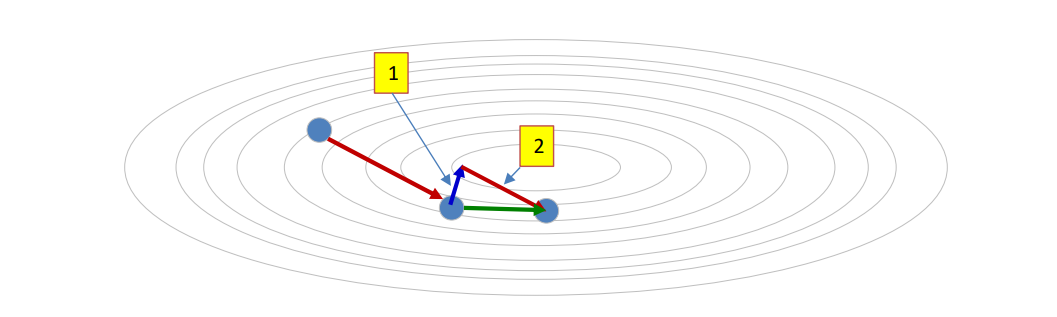
\includegraphics[height=.3\textheight]{pic/momentum_update.png}
        \caption{\footnotesize Momentum update from \url{https://deeplearning.cs.cmu.edu/F24/document/slides/lec6.pdf}}
    \end{figure}
\end{minipage}
\end{frame}

% \begin{frame}{Problem Definition}
%     \begin{itemize}
%         \item \textbf{New Goal}: Automatically adjust the learning rate based on gradient magnitudes to improve convergence, especially in non-convex error surfaces (e.g., in neural networks)
%         \item One of the most famous optimizers that achieves this, is the \textbf{Adam optimizer}
%     \end{itemize}
% \end{frame}

\subsection{AdaGrad}
\begin{frame}{AdaGrad}
       \begin{itemize}
    \item The Adaptive Gradient algorithm, or \textbf{AdaGrad} for short, adjusts the learning rate for each feature based on the cumulative sum of squared gradients
    \item Features that are updated frequently receive a progressively smaller learning rate, allowing sparse features that update slowly to catch up
        \begin{align*}
        G_t &= G_{t-1} + \nabla J(\theta_t) \odot \nabla J(\theta_t) \\
        \theta_{t} &= \theta_{t-1}- \frac{\eta}{\sqrt{G_{t-1}} + \epsilon} \nabla J(\theta_{t-1})
        \end{align*}
        Where:
        \begin{itemize}
            \item $G_t$ is the cumulative sum of squared gradients at time step $t$
            \item $\epsilon$ is a small constant added for numerical stability
        \end{itemize}
    \end{itemize}
\end{frame}

\subsection{RMSProp}
\begin{frame}{RMSProp}
    \begin{itemize}
        \item The problem with AdaGrad is that it becomes incredibly slow. This is because the sum of squared gradients only grows and never shrinks
        \item \textbf{RMSProp} (Root Mean Square Propagation) addresses AdaGrad's slow convergence by introducing a \textbf{decay factor}, allowing only the most recent squared gradients to contribute to the update, which prevents the accumulation of excessively large values

        \begin{align*}
        v_t &= \beta v_{t-1} + (1 - \beta) \nabla J(\theta_t) \odot \nabla J(\theta_t) \\
        \theta_{t} &= \theta_{t-1}- \frac{\eta}{\sqrt{v_{t-1}} + \epsilon} \nabla J(\theta_{t-1})
        \end{align*}
        Where:
        \begin{itemize}
            \item $v_t$ is the \textbf{weighted} cumulative sum of squared gradients at time step $t$ and is equal to the second moment
            \item $\epsilon$ is a small constant added for numerical stability
        \end{itemize}
    \end{itemize}
\end{frame}

\subsection{Adam}
\begin{frame}{Adam}
    \begin{itemize}
        \item Adaptive Moment Estimation, or \textbf{Adam}, combines the concepts of momentum and adaptive learning rates by maintaining an exponentially decaying average of both past gradients and squared gradients
        \item Adam adapts the learning rate for each parameter based on the gradient history: larger gradients lead to smaller update steps, and vice versa
    \end{itemize}
\end{frame}


\begin{frame}{Adam}
    \begin{itemize}
        \item The update rule for Adam optimizer at step $t$ is denoted by $\theta_t$:
        \[\theta_t = \theta_{t-1} - \eta \frac{\hat{m}_{t-1}}{\sqrt{\hat{v}_{t-1}} +\epsilon}\]\\
        \[m_t = \beta_1 m_{t-1} + (1 - \beta_1) \nabla_{\theta} J(\theta_t)\]
        \[v_t = \beta_2 v_{t-1} + (1 - \beta_2) (\nabla_{\theta} J(\theta_t) \odot \nabla J(\theta_t)\]
        \[\hat{m}_t = \frac{m_t}{1 - \beta_1^t}, \quad 
        \hat{v}_t = \frac{v_t}{1 -\beta_2^t}\]
        where:
        \begin{itemize}
            \item $m_t$ and $v_t$ are the first and second moments
            \item $\beta_1$ and $\beta_2$ are decay rates for the first and second moments
            \item $\hat{m_t}$ and $\hat{v_t}$ are bias-corrected estimates of the first and second moments
            \item $\epsilon$ is a small constant to prevent division by zero
        \end{itemize}
    \end{itemize}
\end{frame}

\begin{frame}{Comparison of Momentum Methods}
    \begin{minipage}{0.5\textwidth}
        \centering
        \begin{center}
        \begin{figure}
        \centering
            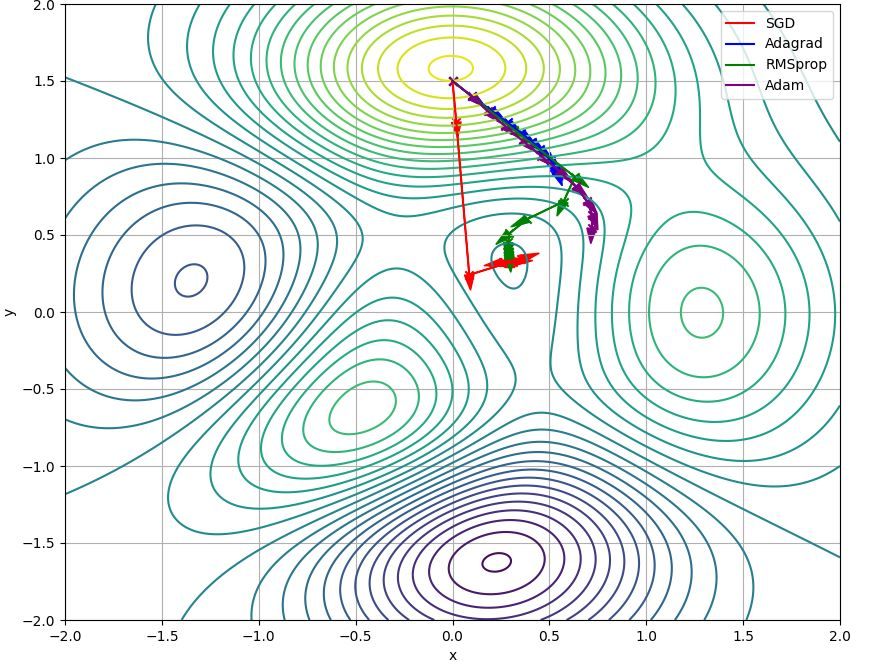
\includegraphics[width=1\linewidth]{pic/all_moment.jpg}
        \end{figure}
        \end{center}
    \end{minipage}%
    \begin{minipage}{0.5\textwidth}
        \centering
        \begin{center}
        \begin{figure}
        \centering
            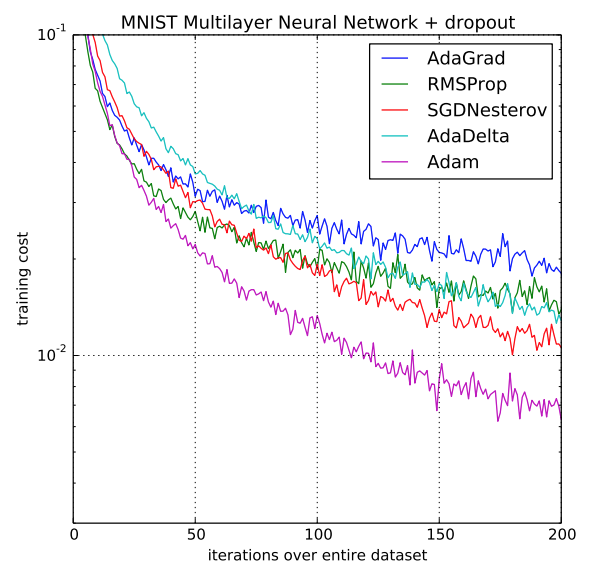
\includegraphics[width=0.8\linewidth]{pic/Adam_training_kingma2015.png}
            \caption{\footnotesize GD comparison on MNIST from \url{kingma2014adam}}
            %\cite{kingma2014adam}
        \end{figure}
        \end{center}
    \end{minipage}
\end{frame}
% \section{References}
% \begin{frame}[allowframebreaks]
%     \bibliography{ref}
%     \bibliographystyle{ieeetr}
%     \nocite{*} % used here because no citation happens in slides
%     % if there are too many try use:
%     % \tiny\bibliographystyle{alpha}
% \end{frame}
\end{document}